\section{Osnovni pojmi za obravnavo zakonov}

Da lahko natančno formuliramo in razumemo zakone, moramo najprej razumeti teoretično ozadje.

\subsection{Proste grupe}

Definicijo zakona \ref{def_zakon_osnovna} lahko bolj formalno zapišemo s pomočjo prostih grup.

\begin{definicija}
\label{def_prosta_grupa}
Naj bo $S$ množica. Grupa $F(S)$ je (do izomorfizma natančno) enolična grupa z lastnostjo, da za poljubno grupo $G$ in poljubno preslikavo
$\varphi: S \to G$ obstaja natanko ena razširitev $\varphi: F(S) \to G$, ki je hkrati homomorfizem grup. 
\end{definicija}

\begin{opomba}
Za poljubni množici $S$ in $T$ velja $F(S) \cong F(T)$ natanko tedaj, ko $\lvert S \rvert = \lvert T \rvert$. Zato lahko v primeru končne množice $\lvert S \rvert = k$ govorimo o 
prosti grupi ranga $k$, ki jo označimo z $F_k$.
\end{opomba}

V viru (\cite[str.~4, tridtev 1.9]{Lyndon_Schupp_2015}) je natančno razloženo znano dejstvo, da lahko elemente proste grupe $F(S)$ predstavimo v obliki okrajšanih besed,
torej besed oblike $w = s_1 \cdots s_n$, kjer je $s_i \in S \cup S^{-1}$ za $i = 1, \ldots, n$ in $s_i \neq s_{i+1}^{-1}$ za $i = 1, \ldots, n-1$. Tu je $S^{-1} = \left\{ s^{-1}  \middle|\, s \in  S \right\}$.
Z upoštevanjem tega dejstva lahko elementom proste grupe $F(S)$ določimo dolžino.

\begin{definicija}
\label{def_dolzina_besede}
Naj bo $w \in  F(S)$ element proste grupe nad množico $S$ in naj bo njegova okrajšana oblika $w = s_1 \cdots s_n$. Potem številu $n$ pravimo dolžina (besede) $w$ in pišemo $l(w) = n$.
\end{definicija}

Brez dokaza bomo privzeli Nielsen--Schreierjev izrek, ki je klasični rezultat v teoriji prosti grup.
TODO navedi vir do dokaza

\begin{izrek}[Nielsen--Schreierjev izrek]
\label{izr_nielsen_schreier}
 Vsaka podgrupa proste grupe je prosta.
\end{izrek}

Ta izrek ima vrsto pomembnih posledic, ena preprostejših -- pa tudi pomembnejših -- je naslednja. 

\begin{posledica}
\label{psl_prosta_grupa_je_torzijsko_prosta}
Proste grupe so torzijsko proste. Z drugimi besedami, vsi elementi razen enote so neskončnega reda. 
\end{posledica}
\begin{dokaz}
Naj bo $w \in F_k \setminus \left\{ 1_{F_k} \right\}$ beseda in $n > 0$ najmanjše število, da velja $w^{n} = 1_{F_k}$. Potem je \begin{equation*}
\langle w \rangle = \left\{ 1_{F_{k}}, w, \ldots ,w^{n-1}\right\} \cong C_n, 
\end{equation*}  
 končne ciklične grupe pa niso proste, s čimer smo prišli v protislovje z Nielsen--Schreierjevim izrekom.  
\end{dokaz}

\subsection{Definicija in osnovne lastnosti zakonov}

Zdaj definiramo izginjajočo množico besede $w$ v grupi $G$.

\begin{definicija}
\label{def_izginjajoca_mnozica}
Naj bo $w \in  F_k$. Potem množico \begin{equation*}
Z(G, w) := \left\{ (g_1, .., g_{k}) \in  G^{k}  \middle|\, w(g_1, \ldots, g_{k}) = 1 \right\} 
\end{equation*}  
imenujemo izginajoča množica besede $w$ v grupi $G$. Tu $1$ označuje enoto v grupi $G$, $w(g_1, \ldots, g_{k})$ pa sliko elementa $w \in F_k = \langle a_{1}, \ldots , a_k \rangle$ s homomorfizmom,
induciranim s preslikavo $\varphi: a_{i} \mapsto g_{i}$ za $i = 1,\ldots, n$ v skladu z definicijo \ref{def_prosta_grupa}.  
\end{definicija}


Zdaj lahko natančno formuliramo definicjo zakona.

\begin{definicija}\label{def_zakon_formalna}
Beseda $w \in F_k$ je $k$-črkovni zakon v grupi $G$, če je $Z(G, w) = G^{k}$. Alternativno, beseda $w \in F_k$ je $k$-črkovni zakon v grupi $G$, če jo vsak homomorfizem $\varphi: F_k \to G$ slika v enoto $1 \in G$.   
\end{definicija}

Definirajmo še zakon v podmnožici grupe.
\begin{definicija}
    \label{def_zakon_v_podmnožici}
    Naj bo $G$ grupa in $H$ njena podmnožica. Beseda $w \in F_k$ je zakon v podmnožici $H$, če za vse izbire $g_1, \ldots, g_k \in H$ velja $w(g_1, \ldots, g_{k}) = 1_G$.
    \end{definicija}
    
    \begin{opomba}
    Beseda $w \in F_k$ je zakon v podmnožici $H \subseteq G$ natanko tedaj, ko je $Z(G, w) \supseteq H^{k}$ ter zakon v vsaki podmnožici $H_1, \ldots, H_n \subseteq G$ natanko tedaj, ko je $Z(G, w) \supseteq \bigcup_{i = 1}^{n} H_i^{k}$.  
    \end{opomba}

Ta definicija nam omogoča vpogled v strukturo zakonov. Naj $K(G, k) \subseteq F_k$ označuje množico $k$-črkovnih zakonov v grupi $G$. Potem v luči prejšnje definicije velja
\begin{equation*}
K(G, k)  = \bigcap_{\varphi: F_k \to G} \ker(\varphi).   
\end{equation*}  
Ta množica je končni presek edink v $G$ in posledično tudi sama edinka. Še več, invariantna je za vsak avtomorfizem $\alpha: F_k \to  F_k$, saj
\begin{equation*}
    K(G, k)  = \bigcap_{\varphi: F_k \to G} \ker(\varphi) = \bigcap_{\varphi: F_k \to G} \ker(\varphi \circ \alpha). 
\end{equation*}  
To je preprosta posledica dejstva, da $\varphi$ preteče grupo $\operatorname{Hom}(F_k, G)$ natanko tedaj, ko jo preteče $\varphi \circ \alpha$.     

\begin{lema}\label{lem_koncni_indeks_koncnega_preseka}
Naj bo $G$ grupa ter $H_1, \ldots, H_n$ njene podgrupe končnega indeksa, torej $[G: H_i] < \infty$ za $i = 1, \ldots, n$. Potem je tudi $\bigcap_{i = 1}^{n} H_i$ podgrupa končnega indeksa v $G$ in velja
\begin{equation*}
\left[ G: \bigcap_{i = 1}^{n} H_i \right]  \le \prod_{i=1}^{n} [G: H_i].  
\end{equation*} 
\end{lema}

\begin{dokaz}
Dovolj je dokazati trditev za $n = 2$, za višje vrednosti sledi z indukcijo. Naj bosta $H_1, H_2 \le G$ podgrupi končnega indeksa, označimo $S: = H_1 \cup H_2$. Naj bosta $C_1$ in $C_2$ množici odsekov podgrup $H_1$ in $H_2$ v $G$ ter naj bo $C$ množica odsekov podgrupe $S$ v $G$. Definiramo preslikavo $f : C \to  C_1 \times C_2$ s predpisom $f(g S ) = (g H_1, g H_2)$. Desna smer sklepa \begin{equation*}
 g S = h S \iff gh^{-1} \in H_1, \, gh^{-1} \in H_2  \iff g H_1 = h H_1, \, g H_2 = h H_2
\end{equation*}  
nam podaja dobro definiranost, leva pa injektivnost preslikave $f$, ki nam da $\lvert C \rvert \le  \lvert C_1 \rvert \lvert C_2 \rvert $.    
\end{dokaz}
Z uporabo te leme direktno sledi, da je grupa $K(k)$ podgrupa končnega indeksa v $F_k$. To dejstvo bo še posebej pobmembno pri iskanju zakonov z računalnikom.

\begin{definicija}\label{def_ozina}
Število \begin{equation*}
\operatorname{girth}_{k}(G) := \min \left\{ l(w)  \middle|\,  w \in F_k \setminus \left\{ 1\right\} \text{ je zakon v } G  \right\} \cup \left\{ \infty\right\} 
\end{equation*}  
je $k$-črkovna dolžina grupe $G$.  
\end{definicija}

% TODO tukaj poveži ožino grafa z bistvom naloge, morda poveži z https://www.researchgate.net/publication/2441748_On_The_Girth_Of_Groups

\begin{definicija}
\label{def_cayleyev_graf}
Naj bo $G$ grupa in $S \subseteq G$ njena podmnožica, za katero velja $S = S^{-1}$. Potem $\operatorname{Cay}(G, S)$ označuje graf z vozlišči $V = G$ in povezavami
$E = \left\{ (p, q) \middle|\, p^{-1}q \in  S \right\}$. Imenujemo ga Cayleyjev graf grupe $G$, generiran z množico $S$.  
\end{definicija}

\begin{opomba}
Pogoj simetričnosti $S = S^{-1}$ nam pove, da je $\operatorname{Cay}(G, S)$ pravi graf in ne zgolj usmerjen. Imamo namreč \begin{equation*}
(p,q) \in  E \iff p^{-1}q \iff q^{-1}p \iff (q,p) \in  E.
\end{equation*}  
\end{opomba}

\begin{primer}
Na spodnjih slikah imamo Cayleyjev graf grupe diedrske grupe $D_{10} = \langle r, Z \rangle$ za različni generatorski množici.
TODO nariši desno od tega še graf s 5 generatorji, morda raje Cayleyjev graf proste grupe F2, saj nastopa naslednji trditvi
\begin{center}
    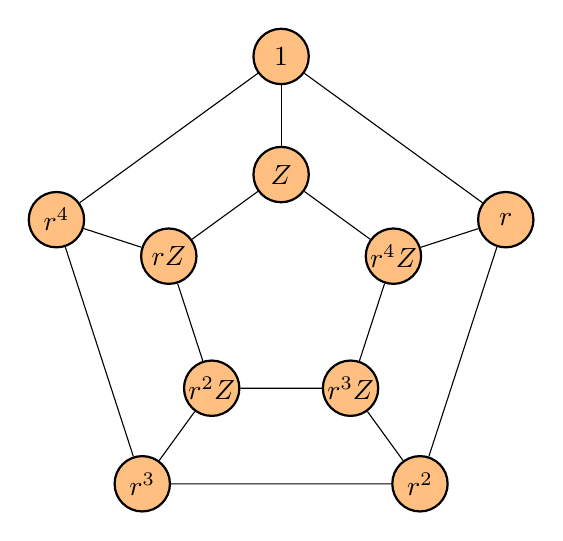
\begin{tikzpicture}[rotate=90, scale=1.5]
    \tikzset{vertex/.style={draw, thick, circle, fill=orange!50, minimum size=20pt, inner sep=0pt}}
    
    \node[vertex] (v1) at (-0*360/5:1) {$Z$};
    \node[vertex] (v2) at (-0*360/5:2) {$1$};
    \node[vertex] (v3) at (-1*360/5:1) {$r^4Z$};
    \node[vertex] (v4) at (-1*360/5:2) {$r$};
    \node[vertex] (v5) at (-2*360/5:1) {$r^3Z$};
    \node[vertex] (v6) at (-2*360/5:2) {$r^2$};
    \node[vertex] (v7) at (-3*360/5:1) {$r^2Z$};
    \node[vertex] (v8) at (-3*360/5:2) {$r^3$};
    \node[vertex] (v9) at (-4*360/5:1) {$rZ$};
    \node[vertex] (v10) at (-4*360/5:2) {$r^4$};
    
    \draw (v1) -- (v2);
    \draw (v1) -- (v3);
    \draw (v2) -- (v4);
    \draw (v3) -- (v4);
    \draw (v3) -- (v5);
    \draw (v4) -- (v6);
    \draw (v5) -- (v6);
    \draw (v5) -- (v7);
    \draw (v6) -- (v8);
    \draw (v7) -- (v8);
    \draw (v1) -- (v9);
    \draw (v7) -- (v9);
    \draw (v2) -- (v10);
    \draw (v8) -- (v10);
    \draw (v9) -- (v10);
    \end{tikzpicture}
    \end{center}
\end{primer}

(TODO dokaz, da je Cayleyjev graf regularen in povezan).

\begin{opomba}
Ime ožina iz definicije \ref{def_ozina} je smiselno v kontekstu definicije Cayleyjevega grafa grupe. TODO zakaj
\end{opomba}


Izkaže se, da so najbolj zanimivi in za obravnavo relevantni dvočrkovni zakoni. To nam sporočata naslednji dve trditvi.
\begin{trditev}
\label{trd_vlozitev_proste_grupe}
 Obstaja vložitev grupe $F_{2 \cdot 3^{k}} = \langle x_1, \ldots, x_{2 \cdot 3^{k}} \rangle$ v grupo $F_2 = \langle x,y \rangle $, da velja $l(x_i) = 2k + 1$, kjer $l(w)$ označuje dolžino besede $w \in F_2 = \langle x,y \rangle$. 
\end{trditev}


\begin{dokaz}
Dokaz trditve ni zahteven, vendar je nekoliko preveč tehničen za potrebe te naloge. Naveden je v~\cite[str.~5]{Schneider_2016}, glavna ideja je obravnavati Cayleyev graf proste grupe $F_2$ z dvema generatorjema.
Drevo vseh besed dolžine $k$ na ustrezen način dopolnimo tako, da dodamo povezave listom. Pri tem dobimo cikle dolžine $2k + 1$ in utemeljimo, da lahko jih lahko obravnavamo kot elemente $F_{2 \cdot 3^{k}}$, vložene v $F_2$. 
\end{dokaz}


\begin{posledica}\label{psl_veccrkovni_zakoni_meje}
Naj bo $G$ grupa in $k \ge 2$ naravno število. Potem velja \begin{equation*}
     \operatorname{girth}_{k}(G) \le  \operatorname{girth}{2}(G) 
\end{equation*}  
in \begin{equation*}
\operatorname{girth}_{2}(G) \le \left( {2 \left\lceil \log_3(\frac{k}{2}) \right\rceil + 1  } \right) \operatorname{girth}_{k}(G).
\end{equation*}  
\end{posledica}
\begin{dokaz}
    Prva neenakost je očitna, saj so vsi dvočrkovni zakoni tudi $k$-črkovni zakoni. Druga neenakost drži, saj lahko po prejšnji trditvi vložimo $F_{{2 \left\lceil \log_3(\frac{k}{2}) \right\rceil}}$ v $F_2$
    tako, da noben generator ni daljši od ${2 \left\lceil \log_3(\frac{k}{2}) \right\rceil + 1  }$. Hkrati velja $F_k \subseteq F_{{2 \left\lceil \log_3(\frac{k}{2}) \right\rceil}}$, kar nam da želeno neenakost.
\end{dokaz}


\subsection{Teorija naključnih sprehodov}

Za obravnavo zakonov v simetričnih grupah bomo potrebovali naključne sprehode, natančneje lene naključne sprehode (TODO poglej, če se res tako imenuje).
Naj bo $G$ grupa, generirana s simetrično podmnožico $S \subseteq G$. Tekom tega razdelka naj bo $\Gamma = \operatorname{Cay}(G, S)$, ki je po prejšnjem premisleku 



\begin{definicija}
\label{def_leni_nakljucni_sprehod}
    Leni naključni sprehod je naključno zaporedje elementov $w_n \in S$ za $n \in \mathbb{N} \cup \left\{ 0\right\} $, porojeno s formulo \begin{equation*}
        \mathbb{P}(w_{n+1} = g   \vert \,  w_n = h) = \begin{cases}
            \frac{1}{2}; & \text{če }  g = h, \\
            \frac{1}{2 \lvert S \rvert }; & \text{če } g = sh \text{ za neki } s \in S.
        \end{cases}
    \end{equation*}  
\end{definicija}
Na vsakem koraku lenega naključnega sprehoda se torej z verjetnostjo $1 / 2$ element ne spremeni, z verjetnostjo $1 / 2$ pa se naključno spremeni v enega od svojih sosedov, ki jih je $\lvert S \rvert$.
To lahko opišemo tudi z matrikami. Recimo, da je $u_n$ vejretnostna porazdelitev $\lvert G \rvert$ razsežnega vektorja, ki predstavlja vozlišča grafa $\Gamma$, po $n$-tem koraku in recimo, da začetno porazdelitev $u_0$ poznamo. Dalje, definiramo matriko lenega naključnega sprehoda $M \in M_{\lvert G \rvert }(\mathbb{R})$, s predpisom    
\begin{equation*}
M = \frac{1}{2} \left(I + \frac{1}{\lvert S \rvert } A \right) = \frac{1}{2} (I + \tilde{A}),
\end{equation*}  
kjer smo z $A$ označili matriko soseščine grafa $\Gamma$, z $\tilde{A}$ pa smo označili matriko $\frac{1}{\lvert S \rvert} A$, da . Ni težko premisliti, da po definiciji \ref{def_leni_nakljucni_sprehod} sledi zveza 
\begin{equation*}
u_n = M^{n} u_0,
\end{equation*}  
ki nam omogoča vpogled v lastnosti naključnih sprehodov. 

\begin{lema}
\label{lem_M_je_sebiadjungirana}
Matrika $M$ je diagonalizabilna, sebiadjungirana in njene lastne vrednosti ležijo v intervalu $[0, 1]$.
\end{lema}
\begin{dokaz}
Ker je realna matrika $M$ simetrična, je diagonalizabilna, sebiadjungirana in velja, da so vektorji, ki pripadajo paroma različnim lastnim vrednostim, med seboj ortogonalni. Enako velja za matriko $A$. Sebiadjungiranost nam implicira realnost lastnih vrednosti matrik $M$ in $A$.
Z oceno matričnih norm \begin{equation*}
    \sqrt{ \lambda_{\max} (\tilde{A}^2)} = \sqrt{\lambda_{\max} (\tilde{A}^{T} \tilde{A} )}  = \lvert\lvert \tilde{A} \rvert\rvert_2 \le \sqrt{\lvert\lvert A \rvert\rvert_1}  \lvert\lvert \tilde{A} \rvert\rvert_{\infty} = 1 
\end{equation*}  
sledi, da ima matrika $\tilde{A}$ lastne vrednosti v intervalu $[-1 ,1]$, kar pomeni, da lastne vrednosti matrike $M$ ležijo v intevalu $[0, 1]$. 
\end{dokaz}

Ker vemo, da so vse lastne vrednosti realne, jih lahko po razvrstimo po velikosti: 
\begin{equation*}
1 \ge \lambda_1(G, S) \ge \lambda_2(G, S) \ge \ldots \ge \lambda_{\lvert G \rvert }(G, S).  
\end{equation*}  
Izkaže se, da je glede na izbiro grupe $G$ in njene generirajoče množice $S$ lastna vrednost $\lambda_1(G, S) = 1 > \lambda_2(G, S)$. (TODO, posledica tega, da je $\Gamma$ povezan + konvergence zaporedja)
Razliko $1 - \lambda_2(G, 2)$ imenujemo \emph{spektralna razlika} grafa $\Gamma$. 

\begin{definicija}
\label{def_diameter_cayleyjevega_grafa}
Diameter Cayleyjevega grafa $\Gamma = \operatorname{Cay}(G, S)$ je število \begin{equation*}
    \operatorname{diam}(G, S) := \min \left\{ n \in \mathbb{N}  \middle|\, \forall g \in G. \exists s_1, \ldots , s_n \in S \cup \left\{ 1_G \right\} . g = s_1 \cdots s_n \right\} 
\end{equation*}  
\end{definicija}
Intuitivno nam diameter Cayleyjevega grafa poda najmanjše število korakov, po katerem lahko naključni sprehod po grafu $\Gamma$ doseže poljubni element grupe $G$. Za vse končnogenerirane in posledično končne grupe je diameter dobro definiran.
Za ocenjevanje dolžin zakonov v grafih je bistvena sledeča zveza med diametrom grafa in spektralno razliko lenega naključnega sprehoda.

\begin{trditev}
\label{trd_zveza_med_diametrom_grafa_in_spektralno_razliko}
 Velja zveza \begin{equation*}
 1 - \lambda_1(G, S) \ge \frac{1}{2 \lvert S \rvert \operatorname{diam}(G, S)^2}.
 \end{equation*}  
\end{trditev}
\begin{dokaz}
% TODO najdi referenco za dokaz te leme, oz si poglej vir, na katerega se sliče Thom
\end{dokaz}

Od tod sledi pomembna posledica \begin{posledica}
\label{psl_posledica_zveze_diameter}
Naj bo vektor $u = \frac{1}{\lvert G \rvert} I$ in naj bo $e_1$ bazni vektor enote $1_G$ (TODO tole bolje razloži). Potem velja ocena \begin{equation*}
\lvert M^{n} e_1 - u \rvert \le \lambda_1(G, S)^{n} \le \left( 1 - \frac{1}{2 \lvert S \rvert \operatorname{diam}(G, S)^2 } \right)^{n}. 
\end{equation*}    
\end{posledica}
\begin{dokaz}
Desna neenakost je direktna posledica trditve \ref{trd_zveza_med_diametrom_grafa_in_spektralno_razliko}. (TODO zakaj leva stran enačbe ... to bi se moralo dati intuitivno dokazati )
\end{dokaz}

Za konec potrebujemo še zadnjo lemo. 
\begin{lema}\label{lem_posledica_neenakosti_csb}
Naj bo $E$ podmnožica grupe $G$ in naj bo $\alpha := \lvert E \rvert / \lvert G \rvert$ in naj bo $(w_n)_{n \in  \mathbb{N}}$ leni naključni sprehod.
Če velja ocena \begin{equation*}
n \ge 2 \lvert S \rvert \operatorname{diam}(G, S)^2 \log(2 \lvert G \rvert ), 
\end{equation*}  
    velja $\mathbb{P}(w_n \in E) \ge \alpha / 2$.
\end{lema}  
\begin{dokaz}
TODO, to je Cauchy--Schwarz
\end{dokaz}

% TOOD tukaj poveži besedilo z intuitivno razloago

Glavni rezultat, ki zagotovi obstoj kratkih zakonov, je Helfgott--Seressov izrek. \begin{izrek}\label{izr_Helfgott_Seress}
Naj par $(\sigma, \tau) \in S_n^2$ generira grupo $S_n$, torej $\langle \sigma, \tau \rangle = S_n$. Potem je diameter grafa $\Gamma = \operatorname{Cay}(S_n, \left\{ \sigma^{\pm 1}, \tau^{\pm 1} \right\} )$ največ 
\begin{equation*}
\exp(C \log(n)^{4} \log(\log(n))).
\end{equation*}
\end{izrek}  
Dokaz tega izreka je zelo težek in se močno nanaša na klasifikacijo končnih enostavnih grup, zato ga opuščamo. Bralec ga lahko najde v \cite{Helfgott_Seress_2013}.
